%% =====================================================================
%%  International Journal of Production Research (IJPR) -- version 2
%%  Taylor & Francis "Interact" layout, APA reference style.
%%
%%  This version supersedes IJPR_CSLAP.tex. It carries the complete,
%%  up-to-date study (multi-instance synthetic benchmark with the
%%  set-partitioning column generation and the LPT anchor, the revised
%%  industrial case with the station-indexed column-generation run, the
%%  temporal hold-out, and the bounded-reassignment sweep).
%%
%%  Compile with the official "Taylor & Francis Interact (APA)" bundle:
%%  keep interact.cls in the working folder (it ships with the template),
%%  together with this file and IJPR_CSLAP.bib. On Overleaf, start from
%%  the "Taylor & Francis Interact (APA reference style)" template and
%%  replace its main.tex and .bib with these two files.
%%
%%  References use BibTeX via apacite (natbibapa), exactly as documented
%%  in the template's main.tex; bibliographystyle = apacite (set below).
%%  Do NOT also load natbib: apacite's natbibapa option provides
%%  \citep / \citet.
%%
%%  Author note: replace the corresponding-author email and the Savoye
%%  city with the final submission details before upload.
%% =====================================================================
% Ensure the "table" option reaches xcolor no matter which package pulls it in
% first (tikz also loads xcolor); this avoids an option clash.
\PassOptionsToPackage{table}{xcolor}
\documentclass[]{interact}

% interact.cls already loads amsmath, amssymb, amsfonts, amsthm, booktabs,
% epsfig, graphicx and rotating. We add only what this manuscript needs.
\usepackage{mathtools}
\usepackage{multirow}
\usepackage{float}
\usepackage{xcolor}  % "table" option passed above; enables \rowcolor/\cellcolor
\usepackage{algorithm}
\usepackage{algpseudocode}
\usepackage{tikz}
\usetikzlibrary{shapes.geometric, arrows.meta, positioning, calc}
\usepackage{url}
\usepackage{hyperref}

% APA references via BibTeX, exactly as the interact-APA sample documents.
\usepackage[natbibapa,nodoi]{apacite}
\setlength\bibhang{12pt}
\renewcommand\bibliographytypesize{\fontsize{10}{12}\selectfont}

\begin{document}

\articletype{RESEARCH ARTICLE}

\title{Efficient and practical solutions for the correlated storage location assignment problem in automated pick-and-pass warehouses}

\author{
\name{Ermal Belul\textsuperscript{a,b}\thanks{CONTACT Ermal Belul. Email: ermalbeluli10@gmail.com},
% ORCID: 0000-0000-0000-0000 (TODO: fill before submission)
Marwane Bouznif\textsuperscript{b},
% ORCID: 0000-0000-0000-0000 (TODO: fill before submission)
Dritan Nace\textsuperscript{a} and
% ORCID: 0000-0000-0000-0000 (TODO: fill before submission)
Antoine Jouglet\textsuperscript{a}}
% ORCID: 0000-0000-0000-0000 (TODO: fill before submission)
\affil{\textsuperscript{a}Universit\'{e} de technologie de Compi\`{e}gne, CNRS, Heudiasyc UMR 7253, Compi\`{e}gne, France; \textsuperscript{b}Savoye, France}
}

\maketitle

% ---------------------------------------------------------------------
% Unstructured abstract (<= 200 words, single paragraph)
% ---------------------------------------------------------------------
\begin{abstract}
Automated, conveyor-driven pick-and-pass warehouses are limited by mechanical station stops rather than by picker travel distance. We study the correlated storage location assignment problem for these systems and replace the usual distance objective with the minimisation of station visits per order, under hard per-station capacity and workload limits. The visit count changes only when a whole order gains or loses a station, and this flat objective stalls branch-and-bound and metaheuristics at scale. Three methods address distinct operational roles: a set-variable reformulation solved by a hybrid local-search engine for strategic re-slotting, a parameter-light clustering heuristic for fast exploratory passes, and a set-partitioning column-generation matheuristic that prices product bundles from one persistent subproblem, removes station symmetry in homogeneous warehouses, and maintains a valid lower bound. Across 29 random instances of 50 to 2,000 stock-keeping units, the set-variable approach is the strongest feasible method and the column generation matches it statistically while never breaching the workload cap. On a real warehouse of 21,874 products the set-variable approach cuts station visits by 13.7\% within every limit, the column generation disturbs the engineered workload balance least, and a bounded reassignment extension maps the trade-off between re-slotting effort and benefit.
\end{abstract}

\begin{keywords}
storage location assignment; pick-and-pass warehouse; warehouse automation; mixed-integer programming; column generation; metaheuristics
\end{keywords}

% =====================================================================
\section{Introduction}
% =====================================================================
Order picking absorbs a large share of warehouse operating cost, so where products sit on the shelves has a direct effect on throughput \citep{xie2024combi}. The correlated storage location assignment problem (CSLAP) chooses that placement by grouping products that are frequently ordered together, with the aim of shortening order preparation. Most CSLAP models pursue this aim by minimising the travel distance of the picker \citep{islam2023}. That objective is the right one when a human walks the aisles. It is the wrong one once the goods move on a conveyor.

In an automated pick-and-pass facility the movement of totes between zones is mechanised. What limits the operation is how often a tote leaves the main line and merges back into it. Each diversion adds a fixed mechanical and handling delay and takes a slot in a finite station buffer. The cost driver becomes the number of station visits per order, together with the balance of workload across zones. We build a CSLAP model on that basis: the objective is the total number of station visits, and no station may exceed its physical capacity or its daily workload budget.

Solving that model at the scale of a real catalogue is the difficulty. The objective counts discrete stops, so its value changes only when a whole order gains or loses a zone. The resulting landscape is flat and piecewise constant, which removes the gradient information that branch-and-bound and local search normally exploit. On instances beyond a few hundred products a standard binary formulation solved by branch-and-bound fails to improve on a feasible starting layout within practical time.

We make three contributions. First, we pose CSLAP for pick-and-pass systems with station visits as the objective and hard capacity and workload limits, give a mixed-integer linear programme for it, and characterise how it behaves computationally: the flat objective reduces the binary branch-and-bound bound to a trivial one and stalls the metaheuristics, while a set-variable reformulation paired with a hybrid local-search engine stays effective up to industrial size. Quality at scale is therefore reported against the best solution found rather than a certified optimum. Second, we develop a set-partitioning column-generation architecture: a station-indexed master with per-station convexity rows, priced from a single persistent subproblem over distinct weighted order supports. For homogeneous warehouses it aggregates into a station-agnostic master that removes label symmetry by construction, and it is driven as a price-and-complete matheuristic that emits a monotone stream of feasible layouts alongside a valid Farley-type lower bound. Third, we benchmark all methods against a genetic algorithm (GA) and simulated annealing with correlated interchange (SA-C) over 29 random instances with paired statistical tests, validate them on a real warehouse of 21,874 products and 26 stations, and add a bounded reassignment extension that caps how many products may move, so the gains can be deployed gradually on an active facility.

Section~\ref{sec:litreview} reviews the relevant production and logistics literature. Section~\ref{sec:model} defines the problem and the decision-aid model. Section~\ref{sec:methods} describes the solution methods. Section~\ref{sec:experiments} reports the synthetic benchmarking and the statistical tests. Section~\ref{sec:industrial} reports the industrial application. Section~\ref{sec:managerial} translates the results into managerial insight, and Section~\ref{sec:perspectives} sets out research perspectives.

% =====================================================================
\section{Related production research}\label{sec:litreview}
% =====================================================================
In a manual warehouse a picker walks to the shelves, so the time to prepare an order follows the distance walked, and storage models minimise that distance \citep{islam2023, wang2020}. In an automated pick-and-pass warehouse a conveyor carries the order past fixed stations and nobody walks, so the model has to minimise something else. \citet{zhang2019cie} model demand correlation explicitly and place co-ordered products near a depot, and \citet{xiao2010correlated} use bill-of-material structure to the same end. These distance models remain the reference point for picker-to-parts settings.

Applying the same objective to automated architectures misreads the cost structure. In robotic mobile fulfilment systems and conveyor systems the goods are transported mechanically, so the system-level limits are the number of station visits, order splits, mechanical dwell, and the synchronisation of workload across zones \citep{azadeh2019, xie2021}. These bottlenecks originate in the per-diversion mechanical setup and in the queueing behaviour of the finite station buffers, both of which fall when an order visits fewer zones \citep{zhu2021, kim2020}. Section~\ref{sec:model} develops this conveyor model.

Recent work supports reframing the objective around discrete touches. \citet{zhu2021} minimise order splits across multiple warehouses by clustering, which maps directly to grouping products into conveyor zones so that an order stays intact. \citet{xie2021} minimise pod-station visits with a mixed-integer programme: in a robotic mobile fulfilment system, robots carry movable shelf racks, called pods, to fixed picking stations, so a pod-station visit is the delivery of one rack to one station, the analogue of our station visit. They prove that fewer visits, combined with dispersed workload, raise system throughput. \citet{mirzaei2021} propose correlated dispersed storage, which spreads correlated items across automated assets to avoid a queue forming at any single workstation. Reducing visits must therefore be paired with workload balance, otherwise the optimisation overloads one zone.

Workload balance belongs in the constraints. \citet{tarczynski2023} give linear-programming models that balance workload across pick-and-pass zones and show that balance is a precondition for reducing total picking time. \citet{pan2015} use a group genetic algorithm to balance zone workload during order batching, and \citet{vanGils2018} show by analysis of variance that storage assignment and zoning have to be optimised together. \citet{boysen2023} survey synchronisation in parts-to-picker systems and conclude that delivering each tote to a capacity-feasible station without queueing is the main determinant of throughput.

Because storage assignment with hard synchronisation is NP-hard, decomposition methods have gained ground. \citet{muter2022} formulate order batching and picker scheduling as a set-partitioning model solved by column generation, with workload pacing enforced inside the pricing problem, and \citet{zhen2025} design column-and-row generation for hard synchronisation constraints in autonomous-robot warehouses. Station capacity and workload can therefore be carried as resource limits inside a pricing subproblem, the route we follow. Two known difficulties of the approach shape our design. A per-order coverage encoding makes the pricing problem scale with the raw order count, and a station-indexed master over identical stations is invariant under relabelling, a symmetry that degrades both the relaxation and the integer search \citep{vanderbeck2000dw}. Our framework prices over distinct weighted order supports and, when stations are interchangeable, aggregates the master so the symmetry never arises. A third difficulty, degeneracy of the covering master, is usually met with dual stabilisation, either boxed dual penalties \citep{dumerle1999stabilized} or weighted dual centres \citep{wentges1997weighted}; we report where it would help rather than implement it, and Section~\ref{sec:cgbound} states exactly what our bound does and does not deliver without it.

Two families of methods sit close to ours and are worth naming, since neither appears among our baselines. Large neighbourhood search repeatedly destroys and repairs part of a solution, and its adaptive form has become a default for routing and assignment problems of this shape \citep{ropke2006alns, pisinger2010lns}; open-source constraint programming over Boolean satisfiability, in particular CP-SAT, is now competitive on set-partitioning models of the kind we solve \citep{perron2023cpsat}. Both would be informative points of comparison, and the local-search engine we use already occupies part of that design space. Learning-based hybrids target the same discrete touches from a different angle: \citet{barnhart2024learnthenoptimize} learn which subproblem to solve next inside a large-scale neighbourhood search for robotic warehousing. That work schedules operations over a short horizon, whereas our decision is the strategic placement that those operations then inherit, so the two are complements rather than competitors.

Table~\ref{tab:litreview} positions this paper against representative studies along the dimensions that matter in the automated setting: the objective, whether a hard per-station workload cap is enforced, the operational environment, the largest reported instance, and the solution method. Several authors already advocate the visit objective. What is missing is a method set that solves it for a real catalogue of tens of thousands of products under hard workload limits and is validated on an operating facility.

\begin{table}[H]
\centering
\tbl{Positioning of this study against representative storage-assignment and order-picking research.}
{\footnotesize\setlength{\tabcolsep}{3pt}
\begin{tabular}{@{}lll>{\raggedright\arraybackslash}p{2.2cm}l>{\raggedright\arraybackslash}p{2.3cm}@{}}
\toprule
Study & Objective & Hard WL cap & Setting & Largest instance & Method \\
\midrule
\citet{zhang2019cie}   & Travel distance       & No    & Manual, correlated      & Hundreds of SKUs & MILP, heuristic \\
\citet{wang2020}       & Travel distance       & No    & Manual picker-to-parts  & Hundreds of SKUs & Clustering \\
\citet{mirzaei2021}    & Dispersion/affinity   & Partial & Robotic fulfilment   & $\sim$10$^3$ SKUs & MIP, policy \\
\citet{xie2021}        & Pod-station visits    & No    & Robotic fulfilment      & $\sim$10$^3$ items & MIP \\
\citet{tarczynski2023} & Picking time          & Yes   & Pick-and-pass           & Small to medium & LP, MILP \\
\citet{muter2022}      & Makespan              & Yes\textsuperscript{a}  & Batching/picking        & Medium & Column generation \\
This study             & Station visits        & Yes   & Pick-and-pass, automated & 21,874 real SKUs & Set-var.\ MILP, CG, heuristic \\
\bottomrule
\end{tabular}}
\tabnote{\textsuperscript{a}Workload enforced as a resource limit inside the pricing subproblem.}
\label{tab:litreview}
\end{table}

% =====================================================================
\section{Problem definition and decision-aid model}\label{sec:model}
% =====================================================================
Table~\ref{tab:notation} collects the notation.

\subsection{The pick-and-pass picking section}
Orders travel along a main conveyor and pass a sequence of picking stations, each on a spur off the main line (Figure~\ref{fig:schematic}). A station holds a fixed set of products on nearby shelving. When an order needs a product stored at a station, its tote diverts onto the spur, an operator picks the required items into the tote, and the tote merges back into the main line. The tote repeats this at every station that holds one of its products, then leaves the section for dispatch. One such diversion is a \emph{station visit}, also called a station stop. An \emph{order split} happens when an order's products sit across more than one station, which forces more than one visit.

\begin{figure}[H]
\centering
\resizebox{\textwidth}{!}{%
\begin{tikzpicture}[
  font=\small,
  station/.style={draw, rounded corners, fill=blue!8, minimum width=1.9cm, minimum height=0.95cm, align=center},
  bin/.style={draw, fill=orange!30, minimum size=0.30cm, inner sep=0pt},
  conv/.style={line width=2pt, -{Latex[length=3mm]}, black!70},
  spur/.style={thick, -{Latex[length=2mm]}, gray!60!black},
]
\draw[line width=6pt, gray!20] (-0.2,0) -- (12.2,0);
\draw[conv] (-0.2,0) -- (12.6,0);
\node[left] at (-0.3,0) {Input};
\node[right] at (12.7,0) {Dispatch};
\node[below, font=\footnotesize] at (6.2,-0.28) {Main conveyor (orders advance in sequence)};
\node[station] (s1) at (2.4,2.25) {Station $s_1$};
\node[station] (s2) at (6.2,2.25) {Station $s_2$};
\node[station] (s3) at (10.0,2.25) {Station $s_{|S|}$};
\node[font=\scriptsize] at (8.2,2.25) {$\cdots$};
\foreach \x in {2.4,6.2,10.0}{
  \draw[spur] (\x-0.65,0.05) -- (\x-0.65,1.75);
  \draw[spur] (\x+0.65,1.75) -- (\x+0.65,0.05);
}
\node[font=\scriptsize, gray!50!black, align=center] at (2.4,1.0) {divert $\uparrow$\\ merge $\downarrow$};
\foreach \x in {0.5,1.4,4.3,8.0,11.4}{ \node[bin] at (\x,0) {}; }
\node[font=\scriptsize, orange!60!black] at (0.5,-0.55) {order tote ($P_o$)};
\node[bin] at (5.55,0.5) {};
\node[bin] at (5.55,0.86) {};
\node[align=center, font=\scriptsize] at (6.2,0.95) {finite\\ buffer};
\draw[step=0.27cm, gray!55, thin] (1.45,2.95) grid (3.35,3.4);
\node[font=\scriptsize] at (2.4,3.62) {shelving: products stored at $s$};
\end{tikzpicture}%
}
\caption{Schematic of a pick-and-pass picking section. A tote diverts onto a station's spur whenever that station stores one of the order's products $P_o$, is processed, then merges back; each diversion is one station visit. Concentrating co-ordered products at a shared station reduces both the number of visits and the occupancy of the finite station buffer.}
\label{fig:schematic}
\end{figure}

Two operational facts drive the model. A visit carries a fixed cost that is independent of how many items are picked, because the tote still has to be decelerated, inducted, scanned, and merged. Grouping co-ordered products at one station therefore collects more items per stop and lowers the visit count. It also decongests the buffer: a station calibrated for 1,000 lines a day handles 500 totes if it serves 500 orders of two lines each, but only 200 totes for the same picking work if it serves 200 orders of five lines. A station buffer also has finite capacity, so too much traffic on one station lets its queue overflow and block the main line. Reducing visits is only safe if the workload on each station stays within a budget. Both effects are captured below: visits in the objective, workload in a hard constraint.

\subsection{Sets, parameters, and decisions}
Let $P$ be the catalogue of products, where each product is one stock-keeping unit (SKU); $O$ the set of orders observed over the planning horizon; and $S$ the set of stations, that is the picking zones. An order $o$ usually requests several products, collected in its line set $P_o \subseteq P$. The same product appears in many orders, and the demand of product $p$, written $L_p$, is the number of order lines in which it occurs over the horizon, in lines per day. Each station $s$ has a number of storage locations $\zeta_s$, a processing speed $V_s$ in lines per day, and a daily time budget $T_s$ expressed as a fraction of a working day. We model the placement at the station level: a product is assigned to exactly one station, and we do not fix which physical slot it occupies, since station shelving can be rearranged without changing the station's total capacity $\zeta_s$. A single station per product keeps inventory and replenishment simple; allowing high-demand products at several stations is left to Section~\ref{sec:perspectives}.

\begin{table}[H]
\centering
\tbl{Notation.}
{\begin{tabular}{@{}cl@{}}
\toprule
Symbol & Definition \\
\midrule
$P,\,O,\,S$ & Sets of products (SKUs), orders, and stations (zones) \\
$P_o$       & Set of products requested in order $o \in O$ \\
$\zeta_s$   & Number of storage locations at station $s$ \\
$L_p$       & Daily order lines for product $p$ (lines per day) \\
$V_s$       & Processing speed of station $s$ (lines per day) \\
$T_s$       & Daily time budget of station $s$ (fraction of a day) \\
$K_s$       & Set of feasible assignment patterns for station $s$ \\
$U,\,w_u$   & Distinct multi-item order supports and their multiplicities \\
$x_{ps}$    & 1 if product $p$ is assigned to station $s$ \\
$z_{os}$    & 1 if order $o$ visits station $s$ \\
\bottomrule
\end{tabular}}
\label{tab:notation}
\end{table}

\subsection{Mixed-integer linear programme}
The binary variable $x_{ps}$ is 1 when product $p$ is assigned to station $s$. The variable $z_{os}$ records whether order $o$ visits station $s$, and it is forced to 1 whenever any product of $o$ sits at $s$. The model is
\begin{align}
\min \quad & \sum_{o \in O} \sum_{s \in S} z_{os} \label{eq:obj}\\
\text{s.t.} \quad
& \sum_{s \in S} x_{ps} = 1 && \forall p \in P \label{eq:assign}\\
& \sum_{p \in P} x_{ps} \le \zeta_s && \forall s \in S \label{eq:cap}\\
& x_{ps} \le z_{os} && \forall o \in O,\ p \in P_o,\ s \in S \label{eq:link}\\
& \sum_{p \in P} x_{ps}\,\frac{L_p}{V_s} \le T_s && \forall s \in S \label{eq:wl}\\
& x_{ps} \in \{0,1\},\quad z_{os} \in [0,1]. && \label{eq:dom}
\end{align}
The objective \eqref{eq:obj} counts station visits across all orders. Constraint \eqref{eq:assign} assigns each product to one station, and \eqref{eq:cap} respects the physical capacity of each station. Constraint \eqref{eq:link} links visits to assignments: if a product of order $o$ is stored at $s$, then $o$ visits $s$. The objective drives $z_{os}$ to its lower bound, so it takes value 1 only when a visit is unavoidable, and it stays integral without a big-$M$ term even though it is declared continuous. Constraint \eqref{eq:wl} caps the daily workload of each station, where $L_p/V_s$ is the time product $p$ adds to station $s$. The workload sum runs over all products assigned to the station, not over a single order.

\subsection{Set-variable reformulation}\label{sec:setvar}
The same model can be expressed with set decision variables rather than a binary matrix \citep{blaisemodeling}. We introduce one set variable $\Phi_s$ per station whose value is the subset of products assigned to that station, so the matrix $x_{ps}$ is replaced by the family $\{\Phi_s\}_{s \in S}$ and the number of declared variables falls from $|P|\times|S|$ to $|S|$. Only the representation changes. The model still decides which of the $|P|$ products goes to which of the $|S|$ stations, and the problem stays NP-hard \citep{garey1979computers}. The gain is practical: a set representation exposes high-level operators (partition, contains, count) and a compact move space, which lets a hybrid local-search engine traverse the flat, piecewise-constant landscape more effectively than flipping $|P|\times|S|$ binary flags one at a time. We solve this reformulation with the Hexaly engine and call it the set-variable approach.

% =====================================================================
\section{Solution methods}\label{sec:methods}
% =====================================================================
Three methods solve the model, one per operational role: the set-variable reformulation of Section~\ref{sec:setvar} for strategic re-slotting, a clustering heuristic for fast exploratory passes, and a set-partitioning column-generation framework for bounded, structurally feasible optimisation. The GA and SA-C baselines of Section~\ref{sec:baselines} provide the comparison.

\subsection{Greedy clustering heuristic}\label{sec:heuristic}
For very large catalogues we use a fast heuristic that builds tightly correlated communities of products and assigns them to stations. It extends the agglomerative idea of \citet{chuang2016}, which merges correlated items into clusters, but it builds disjoint communities by greedy graph connectivity \citep{west2001introduction} and adapts its thresholds to the size of the catalogue, so that a co-occurrence count that signals affinity in a 50-product instance is not mistaken for noise in a 20,000-product one.

Let $N = |P|$. The heuristic needs no per-instance tuning: it fixes four constants, each a fixed fraction of catalogue volume, and derives the operative thresholds from $N$.
\begin{itemize}
\item A \emph{preprocessing frequency floor} $\max(2, \lfloor N/100 \rfloor)$: a product enters the correlation graph only if it appears in at least this many orders. Tying the floor to one\% of the catalogue filters noise at any scale, and the floor of 2 removes single-occurrence products.
\item A \emph{minimum pairwise co-occurrence} $\max(2, \lfloor N/50 \rfloor)$: a pair becomes a candidate edge only when its two products are co-ordered at least this many times, so a retained edge reflects affinity rather than coincidence.
\item A \emph{kept-edge ratio} of $0.1$: a candidate pair survives only if its co-occurrence count is at least a tenth of the more frequent product's own demand, which discards edges that are frequent only because one endpoint is ubiquitous.
\item A \emph{community size bound} $\max(5, \min(15, \lfloor N/20 \rfloor))$: a community holds at most this many products. The bound tracks five\% of the catalogue, clamped between 5 and 15 to match the geometry of a picking zone and to stop a community growing into a block no station can hold.
\end{itemize}
Feasibility is governed by the station capacity $\zeta_s$ rather than by these correlation thresholds, to which the output is robust under moderate variation. The procedure then runs in four stages, summarised in Figure~\ref{fig:heuristic_flow}: filter low-frequency noise and rank correlated pairs; grow disjoint communities from the strongest pair up to the size bound; sweep residual products into their most correlated community with room; then rank communities by demand and place them on stations by historical preference, splitting a community only when no single station can hold it. Appendix~\ref{app:heuristic} states it in full. The heuristic is fast and scalable, but it optimises affinity without the workload constraint \eqref{eq:wl}, so its raw output can breach the workload cap, as the experiments confirm.

\begin{figure}[H]
\centering
\resizebox{0.92\linewidth}{!}{%
\begin{tikzpicture}[
  font=\small,
  node distance=1.1cm and 1.5cm,
  startstop/.style={rectangle, rounded corners, minimum width=3.5cm, minimum height=1cm, text centered, draw=black, fill=red!10},
  process/.style={rectangle, minimum width=4cm, minimum height=1cm, text centered, draw=black, fill=blue!10, align=center},
  decision/.style={diamond, aspect=2, minimum width=3.5cm, minimum height=1cm, text centered, draw=black, fill=green!10, align=center},
  arrow/.style={thick, -{Latex[length=3mm]}}
]
\node (start) [startstop] {Input data ($P,O$) and thresholds};
\node (preproc) [process, below=1cm of start] {\textbf{Step 1: preprocessing}\\filter noise, form valid pairs};
\node (initcomm) [process, below=1cm of preproc] {Initialise community set $\mathcal{C} \leftarrow \emptyset$};
\node (decide1) [decision, below=1cm of initcomm] {Candidate\\pairs left?};
\node (form) [process, right=2cm of decide1] {\textbf{Step 2: community formation}\\greedy expansion of the top pair\\up to the size bound};
\node (post) [process, below=1cm of decide1] {\textbf{Step 3: post-processing}\\assign residual and low-frequency SKUs};
\node (sort) [process, below=1cm of post] {Rank communities by cumulative demand};
\node (decide2) [decision, below=1cm of sort] {Communities\\unassigned?};
\node (assign) [process, right=2cm of decide2] {\textbf{Step 4: station assignment}\\place or split under capacity $\zeta_s$};
\node (end) [startstop, below=1cm of decide2] {Final product-to-station assignment};
\draw [arrow] (start) -- (preproc);
\draw [arrow] (preproc) -- (initcomm);
\draw [arrow] (initcomm) -- (decide1);
\draw [arrow] (decide1) -- node[anchor=south] {yes} (form);
\draw [arrow] (form) |- ($(initcomm.south) + (0,-0.4)$) -| (decide1);
\draw [arrow] (decide1) -- node[anchor=east] {no} (post);
\draw [arrow] (post) -- (sort);
\draw [arrow] (sort) -- (decide2);
\draw [arrow] (decide2) -- node[anchor=south] {yes} (assign);
\draw [arrow] (assign) |- ($(sort.south) + (0,-0.4)$) -| (decide2);
\draw [arrow] (decide2) -- node[anchor=east] {no} (end);
\end{tikzpicture}
}
\caption{Flowchart of the greedy clustering and station-assignment heuristic. Community formation loops until no candidate pairs remain (Steps 1--2); station assignment loops until every community is placed (Steps 3--4).}
\label{fig:heuristic_flow}
\end{figure}

\subsection{Set-partitioning column generation}\label{sec:cg}
Both methods above return a layout, but neither says how far that layout might be from the best one possible. A column-generation framework supplies the missing yardstick, a lower bound on the visit count, while it still produces usable layouts. We build it on a set-partitioning decomposition of the model, following large-scale pricing methods for logistics and scheduling \citep{lubbecke2005selected, desrochers1989column, muter2022}. The general station-indexed master comes first; it handles stations of different sizes and speeds and is the form deployed on the industrial instance of Section~\ref{sec:industrial}. The aggregated reformulation used on the homogeneous synthetic family follows.

\subsubsection{Station-indexed master}\label{sec:cgmaster}
The problem decomposes naturally by station. Recall that $K_s$ is the family of feasible patterns for station $s$: subsets $q \subseteq P$ with $|q| \le \zeta_s$ and $\sum_{p \in q} L_p / V_s \le T_s$. Let $U$ be the set of \emph{distinct} multi-item order supports, each with a weight $w_u$ equal to the number of orders sharing that support; aggregating orders into weighted supports keeps the raw order count out of the master. With one column per station-pattern pair, the pattern cost $c_q = \sum_{u \in U} w_u\,\mathbf{1}[q \cap u \neq \emptyset]$ counts the weighted supports a pattern touches, and the linear master reads
\begin{align}
\min \quad & \sum_{s \in S} \sum_{q \in K_s} c_q\, y_{sq} \notag\\
\text{s.t.} \quad
& \sum_{s \in S} \sum_{q \in K_s:\, p \in q} y_{sq} \ge 1 && \forall p \in P \quad (\sigma_p \ge 0) \label{eq:covergen}\\
& \sum_{q \in K_s} y_{sq} \le 1 && \forall s \in S \quad (\mu_s \le 0) \label{eq:convgen}\\
& 0 \le y_{sq} \le 1 && \forall s \in S,\ q \in K_s. \notag
\end{align}
Constraint \eqref{eq:covergen} covers every product and the convexity rows \eqref{eq:convgen} select at most one pattern per station. For any integer solution whose patterns partition the catalogue, the objective equals the station visits of the multi-item orders exactly, with singleton orders contributing a constant. Pattern feasibility is delegated to pricing: for station $s$, the subproblem minimises the reduced cost $c_q - \sum_{p \in q} \sigma_p - \mu_s$ over patterns satisfying that station's two resource limits. Written with the speed on the right-hand side, those limits are $\sum_{p \in q} 1 \le \zeta_s$ and $\sum_{p \in q} L_p \le T_s V_s$, so the coefficients are the same for every station and only the two right-hand values change. One persistent pricing model therefore serves every station, each call rewriting two numbers. A full pricing pass at one dual vector also yields the per-station Farley-type bound of Section~\ref{sec:cgbound}.

When every station has the same capacity $\zeta$, the same speed $V$, and the same workload cap $T$, the families $K_s$ coincide. Two solutions that differ only in which label sits on which station then describe the same physical layout, and the master cannot tell them apart \citep{vanderbeck2000dw}. The relaxation becomes degenerate, the integer search spends time revisiting relabelled copies of a partition it has already seen, and the $|S|$ pricing calls repeat the same work, since they differ only in the dual $\mu_s$. The aggregation below removes these burdens by construction.

\subsubsection{Aggregated master for homogeneous warehouses}\label{sec:cgagg}
With identical stations and capacity tight, $|P| = |S|\,\zeta$, the problem is exactly a cardinality-constrained set-partitioning problem over station-agnostic product bundles: partition the catalogue into at most $|S|$ bundles of at most $\zeta$ products, and an order visits as many stations as the number of selected bundles its line set touches. A column then needs no station index. Over the current pool $Q'$ of feasible bundles the restricted master is
\begin{align}
\min \quad & \sum_{q \in Q'} c_q\, y_q \notag\\
\text{s.t.} \quad
& \sum_{q \ni p} y_q \ge 1 && \forall p \in P \quad (\sigma_p \ge 0) \label{eq:cover}\\
& \sum_{q \in Q'} y_q \le |S| && (\mu \le 0) \label{eq:card}\\
& 0 \le y_q \le 1 && \forall q \in Q'. \notag
\end{align}
The single cardinality row \eqref{eq:card} condenses the allocation decision into one constraint with one dual $\mu$, which removes the per-station symmetry and the per-station multiplicity of pricing at the source. At integrality under tight capacity the covering rows act as an exact partition into $|S|$ full bundles. Where capacity is slack, the covering inequality together with the visit-minimising objective still returns an exactly-once assignment, since the objective never gains from placing a product in two bundles.

\subsubsection{Pricing subproblem}\label{sec:cgpricing}
One pricing subproblem generates improving bundles. With $a_p \in \{0,1\}$ marking the products of a candidate bundle and $z_u \in [0,1]$ marking the supports it touches (the pattern-level analogue of $z_{os}$), the most negative reduced cost solves
\[
\min\ \sum_{u \in U} w_u\, z_u - \sum_{p \in P} \sigma_p\, a_p - \mu
\qquad \text{s.t.} \quad
z_u \ge a_p\ \ \forall u \in U,\ p \in u, \quad
\sum_{p \in P} a_p \le \zeta, \quad
\sum_{p \in P} L_p\, a_p \le T V, \quad
a_p \in \{0,1\},\ z_u \in [0,1].
\]
The constraint matrix does not depend on the duals, so the pricing model is built once per instance and each call rewrites only the objective coefficients of the $a_p$ variables on a persistent model; the constant $-\mu$ shifts every reduced cost equally and is handled outside the solve. Encoding coverage per distinct support rather than per order keeps the subproblem independent of the raw order count. The gain is large: the 2,000-SKU instances hold between 66,425 and 92,738 distinct supports, a mean of 77,291, against 67,637 to 94,705 raw orders, and the industrial instance of Section~\ref{sec:industrial} reduces 83,183 multi-item orders to 82,224 supports, giving a pricing model of about 98,000 variables and 1.06 million linking rows that is built once and re-priced thereafter. The build is a one-off cost of about 21 seconds, and the first exact solve at 50 SKUs returns in about 0.2 seconds.

\subsubsection{Price-and-complete drive}\label{sec:cgdrive}
Standard column generation adds a single new bundle per iteration, the one with the most negative reduced cost. That loop does not work here. The master selects at most $|S|$ bundles and they must together cover every product, so one new bundle cannot enter any solution until matching bundles for the rest of the catalogue exist as well. Progress stalls even though excellent bundles keep arriving, and the stall comes from the structure of the master rather than from the implementation. We therefore drive the method as a matheuristic: each iteration adds a coordinated set of bundles that forms a full feasible partition, guided by exact pricing and accompanied by the lower bound of Section~\ref{sec:cgbound}. Five components make up the drive.

The warm start is the deterministic longest-processing-time (LPT) partition given to every exact method (Section~\ref{sec:baselines}), polished by a swap descent. The polished partition and randomly mutated feasible variants of it seed the column pool.

The swap descent is a first-improvement search over pairs of products held at different stations. It scores a swap by the exact change in visits plus $\rho$ times the resulting workload overload, that is the total time by which stations exceed their budgets, and accepts the first improving swap it finds before restarting the scan from the new layout. Setting $\rho$ to the total weight of the multi-item supports makes any overload cost more than every visit the swap could save, so a violation is never traded for fewer visits. The change in visits is computed incrementally from per-station support counts rather than by re-scanning the orders (Appendix~\ref{app:swapeval}). Above about 300 products the partner set is sampled to bound the cost of a pass. The descent has three roles: it polishes the warm start, repairs each completed layout, and performs the final polish.

Pricing runs in two steps. A dual-guided greedy step goes first: it considers only products with positive $\sigma_p$, grows a bundle under both resource caps in two orderings (largest dual first, largest dual per unit of workload first), and returns the prefix of that growth at which the reduced cost was lowest, which need not be the full bundle. The exact CPLEX pricer then runs in the same iteration on the persistent model. The greedy step is a cheap source of extra columns and never replaces the exact solve, which alone can prove that no bundle of negative reduced cost remains.

Each priced bundle is then completed into a full feasible partition. Disjoint priced bundles are placed first and the remaining products join, heaviest first, the feasible station of highest co-occurrence affinity, meaning the station whose products already share the most order weight with the product being placed. The descent then refines the completed partition before all of its bundles enter the master together. Only completions that respect both caps are retained, and no bundle that breaks a cap ever enters the master, so the loop emits a stream of deployable layouts and the incumbent never worsens.

The master is finally re-solved with binary variables over the accumulated pool. A product selected in two bundles is kept at the station whose other products share the most order weight with it, a repair that can only lower the visit count. Whichever is better, the layout from the integer master or the best layout found during the loop, is polished for the remaining time. All visit counts we report are recounted directly on the raw orders; we never quote the model's internal objective.

One wall-clock budget per instance is split across these stages: about 8\% goes to the warm-start polish, the generation loop runs until 70\% of the budget has elapsed, the integer master until 85\%, and the final polish takes the remainder. The station-indexed variant of Section~\ref{sec:industrial} follows the same design with a schedule matched to its longer runs: 5\% for the warm-start polish, the generation loop to 62\%, the bound pass to 74\%, the integer master to 82\%, and a final polish that closes the budget. The method runs on IBM CPLEX through its Python interface with one configuration for every instance and size, four threads, and a fixed seed of 42, so a run is reproducible on the same solver version.

\subsubsection{Lower bound and scope}\label{sec:cgbound}
Alongside the layouts, the method computes a number that no layout can beat, a Farley-type lower bound \citep{farley1990note}. It takes the value of the current linear master and subtracts the largest total improvement that the bundles still missing from the pool could bring. How many such bundles there are is what the allocation row states: the aggregated master selects at most $|S|$ of them, and each can improve the objective by at most the most negative reduced cost the pricer reports, so $\mathrm{LB} = z_{\mathrm{RMP}} + |S|\cdot \min(0,\ \mathrm{rc}_{\mathrm{lb}})$, where $\mathrm{rc}_{\mathrm{lb}}$ is the dual bound of the pricing solve, itself a guaranteed floor on the minimum reduced cost. The cardinality dual enters this expression only once, through the constant $-\mu$ that the pricing objective already carries, so it is never counted twice. In the station-indexed master the same argument applies row by row and gives $\mathrm{LB} = z_{\mathrm{RMP}} + \sum_{s \in S} \min(0,\ \mathrm{rc}^{\mathrm{lb}}_s)$.

The bound survives an interrupted pricing call. When a call is cut off by its time slice the solver still reports its own dual bound, which remains a guaranteed floor on the reduced cost, so the bound holds whether or not the call finished. The aggregated solver recomputes it at every iteration and keeps the largest value seen; the station-indexed solver, whose iterations price one station at a time, instead prices all stations once at a common dual vector after the generation loop, which is what its row-by-row formula requires. Convergence is a stronger claim than validity: we declare it only when an exact pricing solve at the true duals proves that no bundle of negative reduced cost is left, so that the linear master is priced out. The covering master admits many equally good dual solutions, which slows how fast the bound rises: the bound can be weak, but it is never wrong.

Within the budgets of Section~\ref{sec:experiments} the bound is informative only at 50 SKUs, where the mean bound of 3,272 sits below the mean of 7,592 visits; from 500 SKUs upward it is vacuous. We therefore present the method as a matheuristic with a valid but loose bound, and dual stabilisation is the lever that would tighten it (Section~\ref{sec:perspectives}). The aggregated form is the reference presentation for homogeneous warehouses and is used on the synthetic family. A heterogeneous site reverts to the station-indexed master, keeping the single persistent pricing model, the price-and-complete drive, and the per-station bound; Section~\ref{sec:industrial} evaluates that configuration.

\subsection{Baselines and initialisation}\label{sec:baselines}
We benchmark against two metaheuristics established in the CSLAP literature: simulated annealing with correlated interchange \citep{kim2012, zhang2019cie} and a genetic algorithm \citep{pan2015}. Because the visit objective is piecewise constant, local swaps rarely change it, so both algorithms evaluate a surrogate that adds capacity and workload penalties to the visit count, plus a dispersion tie-breaker that penalises spreading correlated items. SA-C swaps co-occurring product pairs under a geometric cooling schedule; the GA evolves assignment vectors with quality-proportional selection, swap mutation, and subset crossover, and repairs capacity after each generation. All exact models are seeded with the same feasible start: an LPT assignment that sorts products by frequency and fills the least-loaded station, which satisfies both capacity and workload. The GA and SA-C receive the same start on the synthetic instances. On the industrial case every method starts from the layout the site operates today, so a reported reduction is measured against the configuration actually in use and any difference in final quality reflects the search and not the initialisation. The LPT start also appears in the result tables as a correlation-blind anchor.

% =====================================================================
\section{Computational experiments}\label{sec:experiments}
% =====================================================================
\subsection{Instance generation}
Synthetic instances of $N \in \{50, 500, 1000, 2000\}$ products are adapted from the common-itemset generator of \citet{zhang2019cie}, with a correlation degree of $0.7$ and proportional order volumes. To isolate algorithmic behaviour we model identical stations, with $\zeta_s = \lfloor |P|/|S| \rfloor$ and $V_s = 1$, and set $T_s$ by adding 10\% operational slack to the average workload, so a balanced layout is feasible by construction. The instances reproduce the structure of the industrial data: the synthetic order size, drawn from $U[5,15]$, matches the industrial median of 10 items; the share of co-occurring product pairs is held to a narrow band to match the empirical network sparsity of 2.47\%; and the conditional co-occurrence of the most frequent pairs, at 8.89\%, sits below the industrial value of 14.24\%, so the synthetic data is a conservative test.

\subsection{Protocol and metrics}
The set-variable approach, the GA, SA-C, and the heuristic all use randomised search, so a single run cannot tell whether a ranking reflects method quality or one favourable draw. We therefore evaluate every method over 29 independently generated instances: twelve at 50 SKUs, ten at 500, four at 1,000, and three at 2,000, drawn from the same generator with distinct seeds. Table~\ref{tab:reliability} reports the outcome; a method counts as feasible only when no instance breaches the workload cap. The set-variable approach is the per-instance reference, so each gap is measured against the strongest solution found on the same instance. Across all 29 instances no method violated the slot capacity, so the workload cap is the only binding feasibility signal. No non-trivial certified bound is available at 500 SKUs and beyond: the branch-and-bound bound collapses to the trivial observation that each order visits at least one station, so relative quality is measured against the best solution found.

All optimising methods run under a common per-size wall-clock budget, shown in the Time column of Table~\ref{tab:reliability}: 120, 300, 600, and 1,200 seconds for the four scales. The set-variable approach and the column generation each consume the full budget at every size, so their visit comparison is made at equal computational effort. The GA and SA-C may stop earlier when their own schedules complete, as at 50 and 2,000 SKUs, but never exceed the budget. The heuristic has no time parameter and runs to completion well within it, and the LPT start is immediate. All rankings are conditional on this shared budget and on the hardware used.

\begin{table}[H]
\centering
\tbl{Multi-instance synthetic benchmark with the set-variable approach as the per-instance reference. Mean visits with 95\% confidence interval, mean per-instance gap to the reference, solve time under the common per-size budget, and the share of instances breaching the workload cap. Rows are sorted by mean visits, with the LPT anchor last. The lowest-visit feasible method (no workload violation) in each block is shaded green.}
{\small\setlength{\tabcolsep}{4pt}\begin{tabular}{@{}lrcrrr@{}}
\toprule
Method & Mean visits & 95\% CI & Gap to ref.\ & Time (s) & WL-viol.\ inst. \\
\midrule
\multicolumn{6}{@{}l}{\emph{50 SKUs, 5 stations, 2{,}036 mean orders, $K=12$}}\\
\rowcolor{green!20}
Set-variable MILP & \textbf{7{,}557} & [6{,}828,\ 8{,}286] & (ref) & 120 & 0\% \\
CG (set-part.) & 7{,}592 & [6{,}860,\ 8{,}323] & $+0.5$\% & 120 & 0\% \\
SA-C & 7{,}657 & [6{,}914,\ 8{,}399] & $+1.3$\% & 39 & 0\% \\
Heuristic & 7{,}700 & [6{,}964,\ 8{,}437] & $+2.0$\% & 1 & 100\% \\
GA & 7{,}767 & [7{,}022,\ 8{,}513] & $+2.8$\% & 34 & 0\% \\
Feasible start (LPT) & 8{,}857 & [8{,}054,\ 9{,}661] & $+17.4$\% & $<0.1$ & 0\% \\
\midrule
\multicolumn{6}{@{}l}{\emph{500 SKUs, 5 stations, 20{,}832 mean orders, $K=10$}}\\
\rowcolor{green!20}
Set-variable MILP & \textbf{76{,}041} & [68{,}118,\ 83{,}964] & (ref) & 300 & 0\% \\
CG (set-part.) & 76{,}624 & [68{,}568,\ 84{,}680] & $+0.8$\% & 300 & 0\% \\
Heuristic & 78{,}655 & [70{,}515,\ 86{,}795] & $+3.5$\% & 9 & 80\% \\
GA & 84{,}417 & [75{,}359,\ 93{,}475] & $+11.0$\% & 300 & 0\% \\
SA-C & 88{,}372 & [78{,}937,\ 97{,}808] & $+16.2$\% & 300 & 0\% \\
Feasible start (LPT) & 90{,}177 & [80{,}419,\ 99{,}936] & $+18.5$\% & $<0.1$ & 0\% \\
\midrule
\multicolumn{6}{@{}l}{\emph{1{,}000 SKUs, 10 stations, 38{,}743 mean orders, $K=4$}}\\
\rowcolor{green!20}
CG (set-part.) & 192{,}288 & [149{,}062,\ 235{,}513] & $-0.1$\% & 600 & 0\% \\
Set-variable MILP & \textbf{192{,}330} & [150{,}290,\ 234{,}370] & (ref) & 600 & 0\% \\
Heuristic & 196{,}155 & [151{,}570,\ 240{,}740] & $+1.9$\% & 19 & 100\% \\
GA & 232{,}543 & [182{,}649,\ 282{,}437] & $+21.0$\% & 600 & 0\% \\
SA-C & 241{,}451 & [195{,}307,\ 287{,}594] & $+25.8$\% & 600 & 25\% \\
Feasible start (LPT) & 245{,}228 & [195{,}489,\ 294{,}967] & $+27.7$\% & $<0.1$ & 0\% \\
\midrule
\multicolumn{6}{@{}l}{\emph{2{,}000 SKUs, 20 stations, 78{,}698 mean orders, $K=3$}\textsuperscript{a}}\\
\rowcolor{green!20}
CG (set-part.) & 475{,}035 & [405{,}554,\ 558{,}724] & $-2.4$\% & 1{,}200 & 0\% \\
Heuristic & 483{,}131 & [411{,}517,\ 565{,}068] & $-0.8$\% & 38 & 100\% \\
Set-variable MILP & \textbf{486{,}972} & [410{,}917,\ 568{,}247] & (ref) & 1{,}200 & 0\% \\
GA & 608{,}269 & [520{,}733,\ 731{,}940] & $+24.8$\% & 909 & 0\% \\
SA-C & 614{,}094 & [528{,}037,\ 737{,}715] & $+26.0$\% & 1{,}096 & 0\% \\
Feasible start (LPT) & 621{,}096 & [533{,}942,\ 748{,}257] & $+27.4$\% & $<0.1$ & 0\% \\
\bottomrule
\end{tabular}}
\tabnote{\textsuperscript{a}At $K=3$ the $t$-interval is uninformative; the bracket reports the observed [min, max] range. The set-variable MILP is solved with Hexaly and CG (set-part.) is the aggregated set-partitioning column generation of Section~\ref{sec:cgagg}, solved with CPLEX. ``Gap to ref.''\ is the mean per-instance excess over the reference, so it can differ in sign from the difference of the column means. The feasible start (LPT) is the shared deterministic seed handed to every method, shown as a correlation-blind anchor and excluded from the ranking claims.}
\label{tab:reliability}
\end{table}

\subsection{Results across the instance distribution}\label{sec:reliability}
Three findings hold across the random draws; a fourth, on the column generation, follows below. First, among the heuristic and the literature baselines, the set-variable approach is the best feasible method at every scale, and its margin widens with size: the GA and SA-C trail it by 2.8 and 1.3\% at 50 SKUs, but by 24.8 and 26.0\% at 2,000. A paired Wilcoxon signed-rank test separates the set-variable approach from both baselines at 50 and 500 SKUs ($p = 4.9\times10^{-4}$ and $p = 1.95\times10^{-3}$), and at 1,000 and 2,000 SKUs the paired $t$-test confirms the same ordering, with the Wilcoxon test underpowered at $K=3$ to $4$ and reported descriptively there. Second, the only method in that pool that rivals the reference on raw visits is the heuristic; the difference is not significant at 50 SKUs ($p=0.18$) or at 2,000 ($p=0.5$). The heuristic breaches the workload cap on 80 to 100\% of instances, so it is not usable as it stands. Among the methods that respect the cap, the GA is the stronger baseline from 500 SKUs upward. Third, the variation that matters is the instance draw, not the solver seed: re-running the GA under additional solver seeds gives a within-instance standard deviation of about 1\%, an order of magnitude below the variation between instances.

The mechanisms are visible in the table. The binary formulation solved by branch-and-bound cannot exploit the flat relaxation and, at 1,000 SKUs and above, fails to improve on the LPT seed, so it carries no row. The literature baselines stay feasible but stall on the same flat landscape, where item swaps rarely move the discrete visit count. The heuristic is faster than everything else by more than an order of magnitude, yet it over-clusters correlated items and breaches the cap on most instances. The LPT anchor sits at the opposite corner: it spreads workload most evenly, ignores correlation, and pays the largest visit penalty at every scale.

The column generation adds a fourth reading, with comparisons from exact paired Wilcoxon tests. It is the only method besides the reference with zero workload violations at every size. It trails the reference by 0.5\% at 50 SKUs ($p=0.0015$) and 0.8\% at 500 ($p=0.0039$), matches it at 1,000 while winning three of the four instances, and leads at 2,000 by 2.4\% while winning all three. Pooled over the 29 instances the two methods are statistically indistinguishable ($p=0.11$): the mean per-instance gap is 0.2\% against the reference, while on pooled visit totals the column generation finishes 1.0\% ahead, a difference carried by the largest scales. Pooled, it also dominates every feasible baseline, beating the GA on all 29 instances ($p=2.6\times10^{-6}$), SA-C on 28 of 29 ($p=2.9\times10^{-6}$), and the cap-violating heuristic on 26 of 29 ($p=2.4\times10^{-5}$). Its margin improves monotonically with instance size, and the design choice responsible for that is the one we can isolate. Our earlier implementation kept the station-indexed master and priced with a coverage variable for every raw order, so its cost scaled with the order count times the station count. It stalled beyond 500 SKUs, and on the industrial instance of Section~\ref{sec:industrial} it returned its warm start unchanged after the full ten hours, under both engines we tried. Replacing per-order coverage by the weighted supports of Section~\ref{sec:cgpricing} and aggregating the master removes both factors, and it is what separates a method that finishes at 2,000 SKUs and on a 21,874-product catalogue from one that does not. The two implementations differ in more than that single choice, so we read this as evidence that the aggregation is what makes the decomposition usable at scale, not as a controlled ablation; isolating the remaining components is left to future work (Section~\ref{sec:perspectives}). The reported figures are not budget-starved: on a first-seed instance at each size, extending the column generation well beyond the tabled budget barely moved it, to 86,365 visits at 1,200 seconds for 500 SKUs, 226,566 at 3,600 for 1,000, and 404,882 at 7,200 for 2,000, each within one\% of a shorter run and terminating early on descent convergence.

Three caveats apply. The confidence intervals at 1,000 and 2,000 SKUs ($K=4$ and $3$) are wide and, at 2,000, uninformative, so they are read as ranges. Where an interval carries little information we therefore also report how the instances split, and the splits are unanimous: the reference beats the GA and SA-C on every instance at both sizes, four of four and three of three, and the column generation beats the reference on three of four at 1,000 and three of three at 2,000. A unanimous split across few instances is weaker evidence than a tight interval across many, but it is the evidence these sample sizes support, and it agrees with the ordering the means suggest. The column-generation lower bound is loose at these budgets, so its result stands as a matheuristic reading rather than a certified one. At industrial scale the layout of Section~\ref{sec:industrial} is evaluated on the single available instance, since its size precludes a multi-seed sweep.

% =====================================================================
\section{Industrial application}\label{sec:industrial}
% =====================================================================
We validate the framework on a real warehouse, referred to as Company~A, with $|P| = 21{,}874$ products and 26 stations, 24 of which carry movable SKUs after pruning and enter the solvers and the evaluation. A frequency-based pruning scheme reduces the active decision pool while keeping low-frequency products fixed at their stations and fully accounted for in the capacity bounds. Station geometries and calibrated speeds differ, so absolute workload variance is not comparable across stations. We report the standard deviation of the relative change in each station's utilisation factor; a value near zero means the engineered balance of the site is preserved.

\begin{table}[H]
\centering
\tbl{Industrial case study (Company~A: 21,874 products, 26 stations) under a 10-hour budget. Colour marks the best (green) and runner-up (orange) value in a column, and workload violations (red); the legacy row is shaded.}
{\small\setlength{\tabcolsep}{4pt}\begin{tabular}{@{}lrrrrrr@{}}
\toprule
Method & Visits & Rel.\ dev.\ (\%) & Time (s) & Max WL & Std dev util.\ (\%) & Viol. \\
\midrule
\rowcolor{yellow!50!black}
\textcolor{white}{Original layout (A)} & \textcolor{white}{1{,}062{,}507} & \textcolor{white}{15.81} & \textcolor{white}{0} & \textcolor{white}{9{,}923} & \cellcolor{green!80!black}\textcolor{white}{0.00} & \textcolor{white}{None} \\
Heuristic & 1{,}016{,}003 & 10.74 & \cellcolor{blue!12}\textbf{94} & \textcolor{red}{\textbf{11{,}919}} & 37.09 & \textcolor{red}{\textbf{WL}} \\
Set-variable MILP & \textcolor{green!60!black}{\textbf{917{,}465}} & 0.00 & 36{,}000 & 10{,}467 & \textcolor{orange!90!black}{\textbf{4.48}} & None \\
CG (station-indexed) & \textcolor{orange!90!black}{\textbf{1{,}000{,}844}} & 9.09 & 36{,}000 & 10{,}074 & \textcolor{green!60!black}{\textbf{2.41}} & None \\
GA & 1{,}046{,}071 & 14.02 & 19{,}358 & \textcolor{red}{\textbf{10{,}972}} & 18.52 & \textcolor{red}{\textbf{WL}} \\
SA-C & 1{,}058{,}563 & 15.38 & 36{,}000 & 10{,}811 & 12.14 & \textcolor{red}{\textbf{WL}}\textsuperscript{a} \\
\bottomrule
\end{tabular}}
\tabnote{Max WL is the busiest station's realised daily load in lines. The site tolerates up to $+10\%$ over each station's legacy load; the busiest legacy station carries 9,923 lines, so its bound is 10,915, and the check is per station (a Max WL below 10,915 need not certify feasibility). Time $36{,}000$\,s is the full ten-hour budget. Set-variable MILP: Hexaly; CG: station-indexed master (Section~\ref{sec:cgmaster}), CPLEX.}
\tabnote{\textsuperscript{a}SA-C's per-station loads were not retained, so its violation flag is set conservatively.}
\label{tab:industrial}
\end{table}

Table~\ref{tab:industrial} confirms the synthetic findings on the operating site. The heuristic is again fast and again infeasible: it runs in 94 seconds and removes 46,504 visits, but it pushes several stations far past their engineered limits (Figure~\ref{fig:wl_heur}), so its raw output would congest those stations if deployed without a balancing pass. The binary formulation under branch-and-bound does not improve on the original layout within the limit and carries no row. The set-variable approach lowers station visits from 1,062,507 to 917,465, a reduction of 145,042 visits or 13.7\%, while holding the standard deviation of the relative utilisation change to 4.48 and each station's shift within $[-5.9\%, +9.6\%]$, inside the 10\% slack of the site (Figure~\ref{fig:wl_milp}). Its advantage comes from the set reformulation and from a hybrid architecture that pairs local search with exact methods, which suits the flat search space that defeats branch-and-bound.

\begin{figure}[H]
\centering
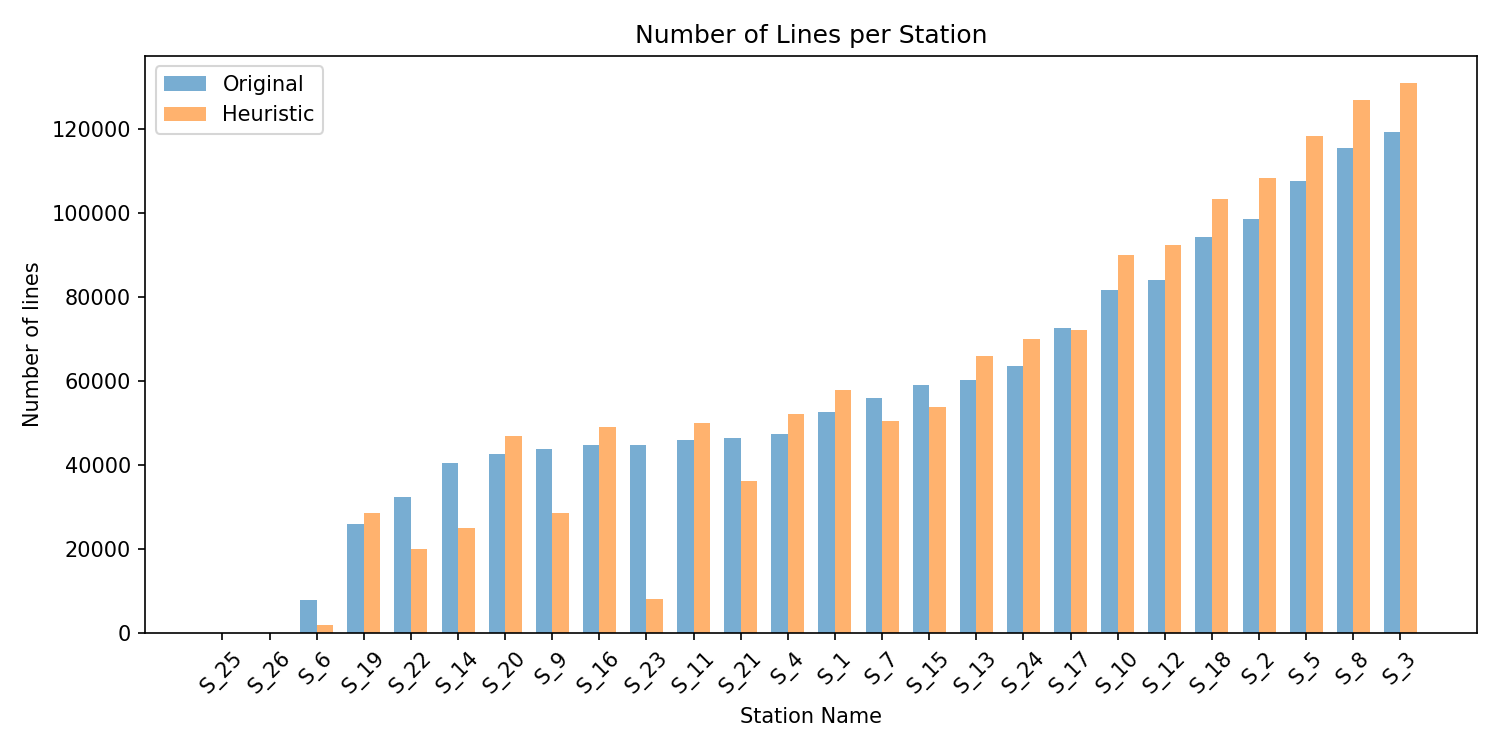
\includegraphics[width=0.49\linewidth]{Images_CSLAP/r4_number_of_lines_per_station.png}\hfill
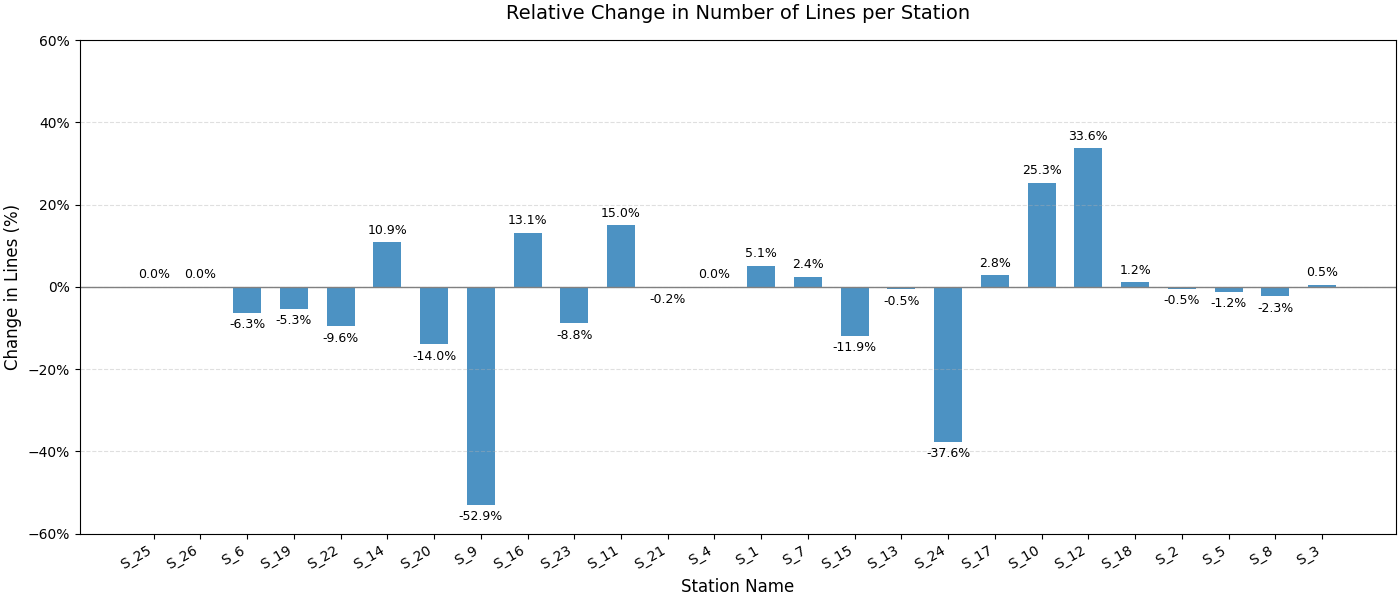
\includegraphics[width=0.49\linewidth]{Images_CSLAP/r5_pct_change_lines_per_station.png}
\caption{Lines per station (left) and relative change in utilisation (right) for the heuristic layout against the original. Several stations move well past their capacity.}
\label{fig:wl_heur}
\end{figure}

\begin{figure}[H]
\centering
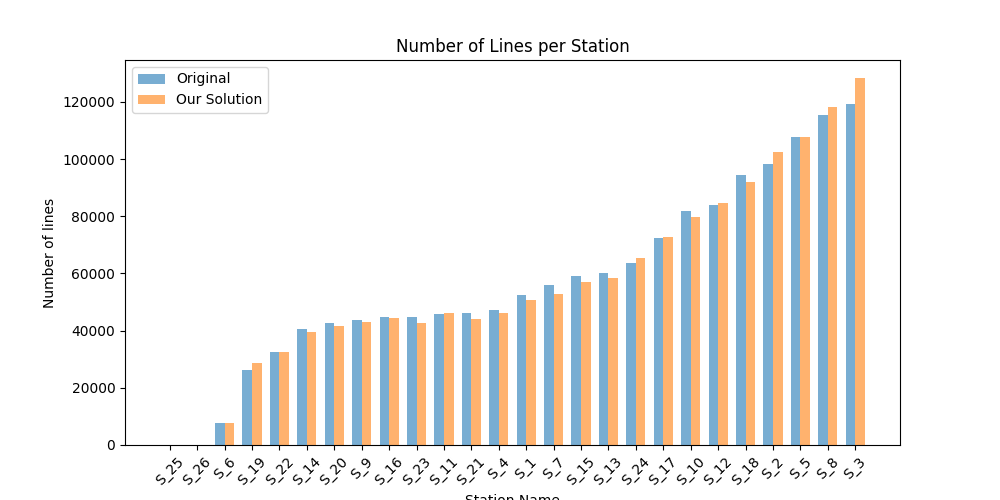
\includegraphics[width=0.49\linewidth]{Images_CSLAP/Hexaly_number_of_lines_per_station.png}\hfill
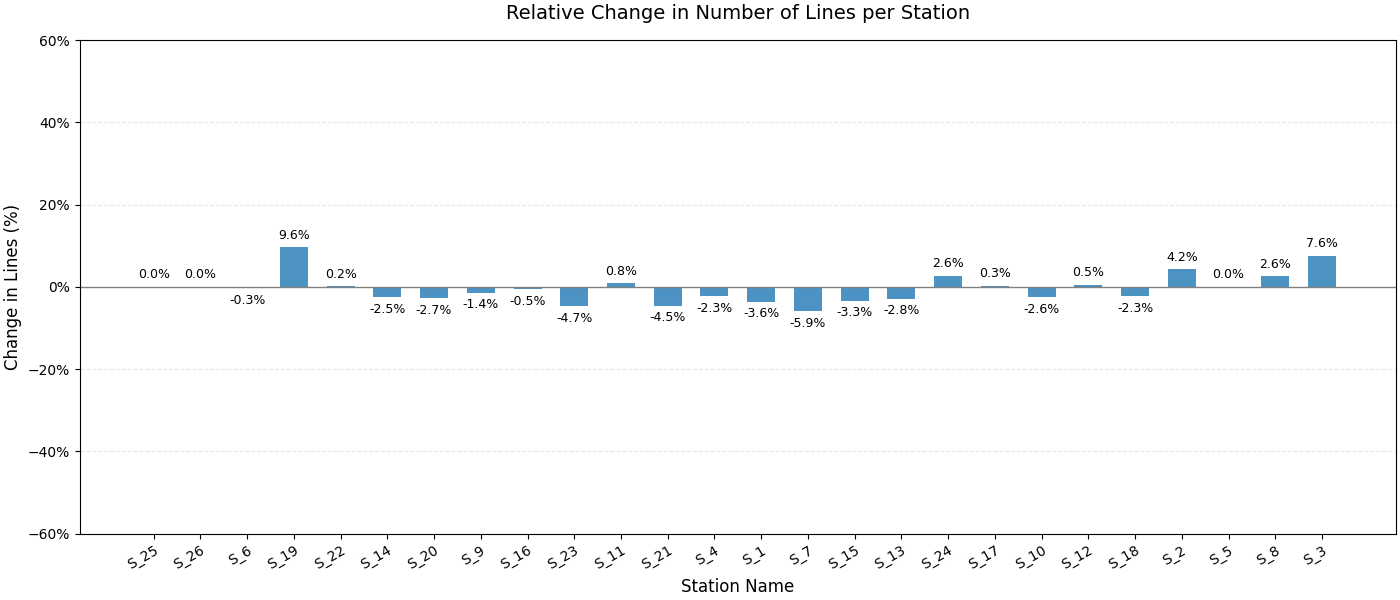
\includegraphics[width=0.49\linewidth]{Images_CSLAP/Hexaly_pt_relative_change_number_of_lines_per_station.png}
\caption{Lines per station (left) and relative change in utilisation (right) for the set-variable layout against the original. The relative change stays inside the operational slack on every station.}
\label{fig:wl_milp}
\end{figure}

\begin{figure}[H]
\centering
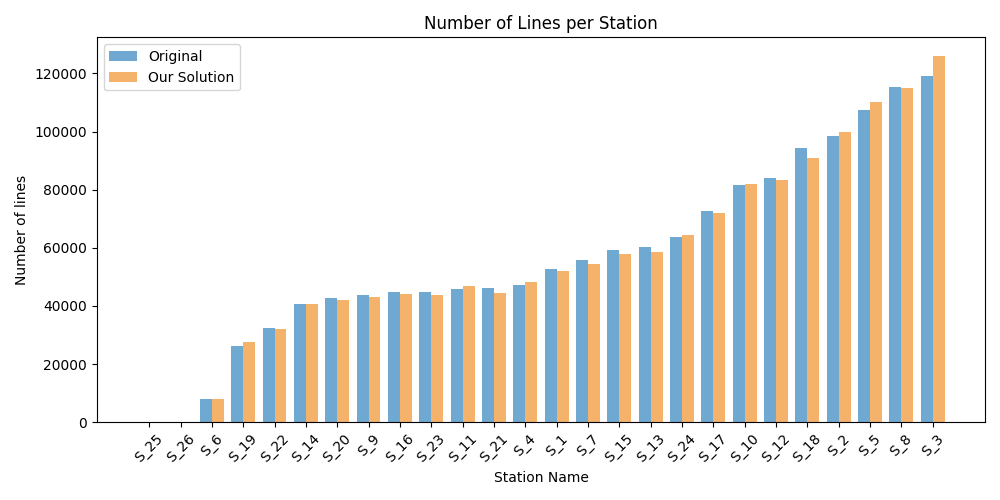
\includegraphics[width=0.49\linewidth]{Images_CSLAP/CG_SetPart_number_of_lines_per_station.png}\hfill
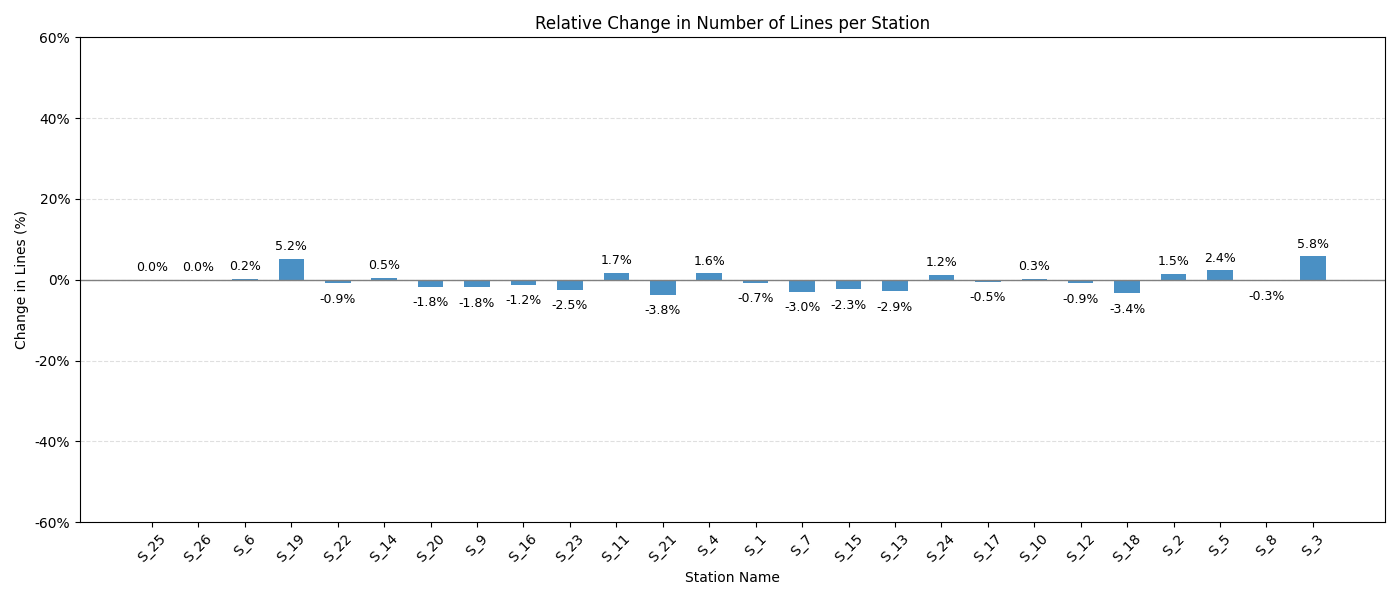
\includegraphics[width=0.49\linewidth]{Images_CSLAP/CG_SetPart_pt_relative_change_number_of_lines_per_station.png}
\caption{Lines per station (left) and relative change in utilisation (right) for the station-indexed column-generation layout against the original. The station loads track the engineered legacy balance almost identically.}
\label{fig:wl_cg}
\end{figure}

The column generation ran on Company~A in its station-indexed form with the set-variable approach's inputs: the same per-station workload caps, the same workload basis, and the same full evaluation, so the two methods solve the same constrained problem. Each active station keeps its own convexity row, and the single persistent pricing model serves all of them by swapping the two station-dependent right-hand sides per call. Two elements differ from the homogeneous drive. The warm start is the layout the site operates today rather than an LPT partition, so the run improves the live configuration step by step. Priced bundles are installed into that incumbent by an ejection-style recompletion that evicts the bundle's products, rebuilds the target station, and reinserts the displaced products by co-occurrence affinity, instead of rebuilding a partition from scratch. The swap descent keeps the acceptance rule of Section~\ref{sec:cgdrive}, with the workload change of a move measured against each station's own speed. Over 106 iterations the run generated 2,670 columns with exact pricing throughout and used 35,940 of the 36,000 seconds, improving the pruned-instance objective from the 680,270-visit warm start to 627,523. On the full evaluation the layout scores 1,000,844 visits: 9.09\% above the set-variable solution, and 5.8\% below the live legacy layout, or 61,663 fewer visits.

Three properties stand out. The layout is strictly feasible with the same violation profile as the set-variable solution: both exceed the raw legacy load on ten stations, and both stay within the site's 10\% tolerance on every one, with the column-generation deviations spanning $[-3.8\%, +5.8\%]$ against $[-5.9\%, +9.6\%]$ for the set-variable layout. It disturbs the engineered utilisation balance least among the optimising methods, at a standard deviation of 2.41 against 4.48 and 12.14 (Figure~\ref{fig:wl_cg}). It also completes and improves at a scale where a conventional drive of the same decomposition, one pricing model per station with a coverage variable per order, returned its warm start unchanged under the same ten-hour budget. The Farley pass ran to completion but stays uninformative at this scale, consistent with Section~\ref{sec:cgbound}. The site therefore has two deployment profiles: the set-variable approach when the deepest visit reduction is the goal, and the column generation when operations want an improvement that barely moves the engineered balance.

Over the 66-day quarter in the dataset, the original layout required 1,062,507 visits, about 16,099 stops per day; the set-variable layout removes about 2,198 stops per day. Multiplying the 145,042 eliminated visits by a fixed mechanical time per visit frees roughly nine working days of picker and conveyor dwell per quarter. The projection is linear and ignores queueing, so a discrete-event study is needed to confirm it (Section~\ref{sec:perspectives}). As a planning figure it still gives operations a concrete target.

\subsection{Robustness on unseen weeks}
A layout is optimised once and then operated as demand evolves, so we test out of sample. The dataset spans 13 weeks. In the first test the model sees only the first 10 weeks and is evaluated on the last 3; in the second it sees the first 8 and is evaluated on the last 5. Each layout is compared with the original placement and with an oracle layout optimised directly on the test weeks with perfect knowledge (Table~\ref{tab:temporal}). This out-of-sample design follows robustness practice in storage assignment, where an implementable policy is contrasted with a perfect-information oracle \citep{lee2020cie, wang2020}. Using 10 weeks of history cuts visits by 6.6\% on the held-out weeks, against 12.1\% for the oracle; using 8 weeks cuts visits by 7.4\%, against 10.2\%. The recent past therefore captures most of the structural affinity benefit, enough for a durable gain on this site. That stability may not carry to more volatile assortments, where combining the model with demand prediction is an open route.

\begin{table}[H]
\centering
\tbl{Out-of-sample station-visit performance on held-out weeks.}
{\begin{tabular}{@{}llrr@{}}
\toprule
Test period & Layout (training period) & Total visits & Mean visits \\
\midrule
\multirow{3}{*}{Last 3 weeks}
 & Original placement & 265{,}876 & 4.052 \\
 & Optimised on first 10 weeks & 248{,}358 & 3.785 \\
 & Oracle (optimised on last 3 weeks) & 233{,}728 & 3.562 \\
\midrule
\multirow{3}{*}{Last 5 weeks}
 & Original placement & 423{,}593 & 3.926 \\
 & Optimised on first 8 weeks & 392{,}318 & 3.636 \\
 & Oracle (optimised on last 5 weeks) & 380{,}356 & 3.525 \\
\bottomrule
\end{tabular}}
\label{tab:temporal}
\end{table}

\subsection{Bounded reassignment}\label{sec:reassign}
An established facility cannot absorb a disruptive re-slotting wave \citep{chabot2024reassignment}, so we bound how many products may move. Let $s'(p)$ be the legacy station of product $p$. Adding the single constraint
\begin{equation}
\sum_{p \in P} x_{p,\,s'(p)} \ \ge\ |P| - k
\label{eq:reassign}
\end{equation}
limits the number of relocated products to at most $k$. Nothing else changes: the objective \eqref{eq:obj}, the capacity rows \eqref{eq:cap} and the workload rows \eqref{eq:wl} are those of Section~\ref{sec:model}, and the legacy layout stays feasible for every $k$, so the model has a solution whatever budget the site sets. We solve it with the set-variable engine for $k \in \{250, 500, 1000, 2000, 5000\}$ under a one-hour budget each, and contrast the result with the legacy layout ($k=0$) and with the full re-optimisation that reached 917,465 visits under a 10-hour budget (Table~\ref{tab:reassign}, Figure~\ref{fig:ksweep}). The same limit fits the column-generation framework without changing its structure: counting, for each bundle, how many of its products would leave their legacy station turns \eqref{eq:reassign} into one knapsack-style row over the bundle variables, whose dual then enters pricing as a per-product penalty for moving a product away from where it sits today. We have not run that variant, and report the bounded results from the set-variable engine alone.

\begin{table}[H]
\centering
\tbl{Bounded-reassignment trade-off on the industrial instance. ``\% of full benefit'' is the reduction relative to the 145,042-visit full re-optimisation; the last column counts stations exceeding their cap.}
{\small\begin{tabular}{@{}lrrrrr@{}}
\toprule
Relocation cap & \% catalogue & Total visits & Reduction & \% of full benefit & WL-viol.\ stations \\
\midrule
Legacy ($k=0$) & 0\% & 1{,}062{,}507 & -- & -- & 0 \\
$k=250$        & 1.1\% & 1{,}061{,}302 & 1{,}205 & 0.8\% & 0 \\
$k=500$        & 2.3\% & 1{,}060{,}120 & 2{,}387 & 1.6\% & 0 \\
$k=1{,}000$    & 4.6\% & 1{,}056{,}412 & 6{,}095 & 4.2\% & 0 \\
$k=2{,}000$    & 9.1\% & 1{,}049{,}730 & 12{,}777 & 8.8\% & 0 \\
$k=5{,}000$    & 22.9\% & 1{,}034{,}735 & 27{,}772 & 19.2\% & 0 \\
Full re-opt.   & --     & 917{,}465 & 145{,}042 & 100\% & 0 \\
\bottomrule
\end{tabular}}
\label{tab:reassign}
\end{table}

\begin{figure}[H]
\centering
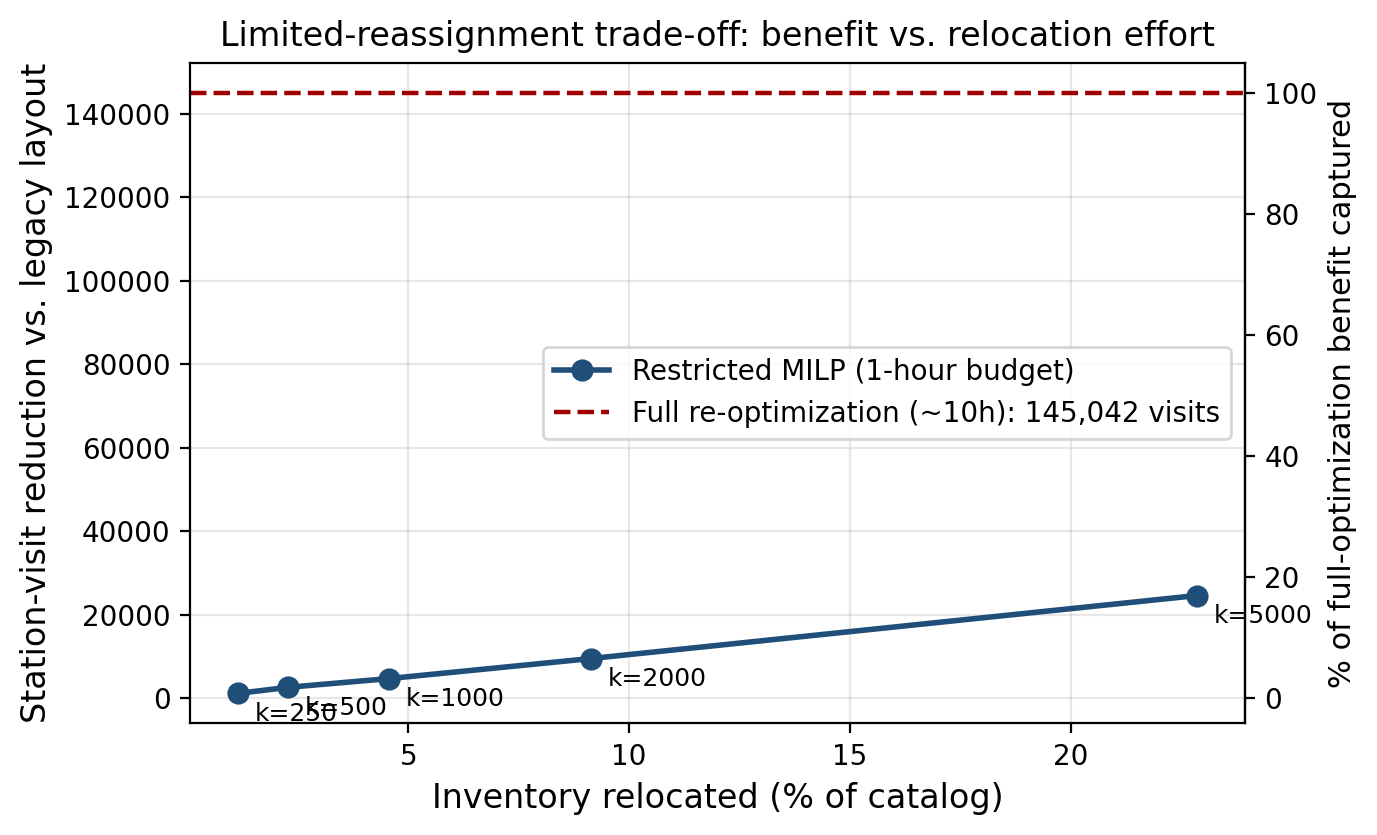
\includegraphics[width=0.7\linewidth]{Images_CSLAP/reassignment_ksweep_curve.png}
\caption{Station-visit reduction against the share of the catalogue relocated. The dashed line marks the full re-optimisation benefit, which accrues gradually with relocation effort.}
\label{fig:ksweep}
\end{figure}

Two findings emerge. The benefit of bounded re-slotting accrues roughly in step with the relocation effort: relocating 2.3\% of the catalogue captures 1.6\% of the full reduction, and relocating 22.9\% captures 19.2\%. No small subset of moves captures a disproportionate share, so most of the gain in the full solution still comes from a large rearrangement that a tight budget cannot reproduce. The curve quantifies what a manager gives up by limiting disruption, and lets the budget $k$ be matched to available labour against a known marginal benefit. Every bounded layout also stays feasible: at each cap the solver keeps all stations within both capacity and workload, and the busiest station load and the spread of utilisation barely move from their legacy values. The whole curve can therefore be deployed as it stands, because each station's residual time budget is reserved for the frozen low-frequency products before the bounded search runs.

% =====================================================================
\section{Managerial insights for decision makers in industry}\label{sec:managerial}
% =====================================================================
The results carry five messages for warehouse operations.

Track station visits as a slotting indicator. Each diversion generates mechanical queueing and handling delay, so stops per order expose congestion that a distance metric hides. On Company~A the set-variable layout removes 13.7\% of the visits, about 2,198 stops a day.

Read the labour effect as a planning figure. The nine working days of dwell freed per quarter (Section~\ref{sec:industrial}) follow from a fixed time per visit and no queue model, so a discrete-event study is needed before the figure is booked as a saving. It is still a concrete target for operations.

Match the tool to the decision. For a scheduled quarterly re-slotting, the set-variable approach gives the best layout we obtain while holding every station within capacity. When the priority is an improvement that barely moves the engineered workload balance, the column generation delivers a 5.8\% visit reduction with the smallest utilisation disturbance of any optimising method, and it never breached a workload cap in any experiment. For a fast exploratory pass, the clustering heuristic runs in seconds, provided its raw output is filtered for workload before use.

Improve continuously without a shutdown. The bounded-reassignment model lets a site move only as many products as its workforce can handle in one cycle. Table~\ref{tab:reassign} gives the trade-off curve directly, so the relocation budget can be set against the marginal benefit rather than guessed, and every point on that curve holds all stations within capacity and workload.

Recalibrate on a rolling window. A layout optimised on the most recent 8 to 10 weeks of orders captures most of the attainable benefit on the following month. Re-optimising at that cadence keeps the layout current with limited engineering effort, and the reassignment cap keeps each cycle non-disruptive.

% =====================================================================
\section{Research perspectives}\label{sec:perspectives}
% =====================================================================
Four tracks extend this work. The first concerns the column generation. Dual stabilisation, for instance the boxed dual penalties of \citet{dumerle1999stabilized} or the weighted dual centres of \citet{wentges1997weighted}, would tighten the Farley bound that is currently loose at scale and turn the matheuristic reading into certified gaps. A branch-and-price layer on top of the price-and-complete drive would then let the bound and the primal search close the remaining distance. On the industrial side, the station-indexed run improves the live layout feasibly but trails the set-variable solution by 9.09\% on visits; a longer horizon, or hybridising the swap descent with the set-variable engine, would close that gap.

The second track is a fuller experimental account of the drive itself. We report the effect of the design choice that governs scale, the move from per-order to support-level pricing, because we have runs on both sides of it, but the contribution of each remaining component, the dual-guided greedy step, the completion policy and the final descent, would need a controlled ablation with one component disabled at a time under the budgets of Table~\ref{tab:reliability}. The same protocol should carry an adaptive large neighbourhood search and an open-source constraint-programming model \citep{ropke2006alns, perron2023cpsat} as additional baselines, which would tell a practitioner without a commercial licence what the approach costs in solution quality.

The third track is product geometry. The model counts a product as one unit of a station's capacity. Replacing that count with a per-product footprint $f_p$ in constraint \eqref{eq:cap}, coupled to the temporal budget \eqref{eq:wl}, would let three-dimensional packing limits enter without changing the structure of the programme. The same extension covers duplicating a high-demand product across several stations, which the single-station assumption of Section~\ref{sec:model} currently excludes. In the decomposition that change is contained: the covering rows \eqref{eq:cover} already allow a product in several selected bundles, so the equality that ties each product to one station is what has to be relaxed, to an upper limit on the number of stations a product may occupy, with the replenishment cost of each extra copy charged in the pattern cost so that pricing only proposes a duplicate when the visits it saves outweigh it.

The fourth track is the visit-to-throughput link. We balance workload, which lowers expected queueing, but we do not yet model the queue. Feeding the optimised layouts into a discrete-event simulation would quantify queue states and convert the planning figures of Section~\ref{sec:managerial} into measured throughput, and would open the door to stochastic demand and real-time routing.

% =====================================================================
\section{Conclusion}\label{sec:conclusion}
% =====================================================================
We posed the correlated storage location assignment problem for automated pick-and-pass warehouses with station visits as the objective and hard capacity and workload limits. The objective is piecewise constant, which stalls branch-and-bound and metaheuristic search at scale. Two routes clear that barrier. A set-variable reformulation paired with a hybrid local-search engine gives the best feasible layouts across synthetic instances of 50 to 2,000 products, with a margin over the literature baselines that widens with size, and lowers station visits on a real 21,874-product warehouse by 13.7\% while keeping every station within capacity. A set-partitioning column generation, priced from one persistent subproblem over weighted order supports and driven as a price-and-complete matheuristic, matches that reference statistically on the synthetic family, never breaches a workload cap, carries a valid lower bound, and on the industrial site improves the live layout by 5.8\% while disturbing the engineered workload balance least. A bounded-reassignment extension maps the trade-off between re-slotting effort and benefit, which makes the gains deployable on an active site without a shutdown.

% ---------------------------------------------------------------------
% BACK MATTER (IJPR order)
% ---------------------------------------------------------------------
\section*{Author contributions}
The authors confirm contribution to the paper as follows. Ermal Belul, Marwane Bouznif, Dritan Nace, and Antoine Jouglet were involved in the conception, design, and modelling of the framework; Ermal Belul developed the software and analysed the empirical data; Ermal Belul drafted the manuscript, and Marwane Bouznif, Dritan Nace, and Antoine Jouglet critically revised it for intellectual content. All authors gave final approval of the version to be published and agree to be accountable for all aspects of the work.

\section*{Acknowledgements}
The authors thank the operational teams at Company~A for the dataset and for their insight into the picking process, and Savoye and the Universit\'{e} de technologie de Compi\`{e}gne for hosting the work.

\section*{Funding details}
This work was supported by the Association Nationale de la Recherche et de la Technologie (ANRT) under a CIFRE doctoral grant [grant number: TODO-CIFRE-NUMBER] in partnership with Savoye.

\section*{Disclosure statement}
The authors report there are no competing interests to declare.

\section*{Declaration of generative AI use}
During the preparation of this work the authors used a generative AI assistant to refine language and improve readability. After using this tool the authors reviewed and edited the content as needed and take full responsibility for the content of the published article.

\section*{Notes on contributors}
\textit{Ermal Belul} is a doctoral researcher at the Universit\'{e} de technologie de Compi\`{e}gne (Heudiasyc laboratory) and Savoye, working on decision-support tools under uncertainty for intralogistics, with a focus on storage assignment and warehouse optimisation.

\textit{Marwane Bouznif} is a research and development engineer at Savoye, working on optimisation methods for automated warehouse systems.

\textit{Dritan Nace} is a professor at the Universit\'{e} de technologie de Compi\`{e}gne (Heudiasyc laboratory). His research covers combinatorial optimisation, network design, and robust optimisation.

\textit{Antoine Jouglet} is a professor at the Universit\'{e} de technologie de Compi\`{e}gne (Heudiasyc laboratory). His research covers scheduling, constraint programming, and combinatorial optimisation.

\section*{Data availability statement}
This journal applies the Taylor \& Francis ``share upon reasonable request'' data sharing policy. The 29 synthetic benchmark instances used in the computational experiments are \href{https://anonymous.4open.science/r/Anonymized_Export_CSLAP_v2-01BC/README.md}{openly available online} with the seeds and generator settings that produced them, so the instance set can be reconstructed exactly; the de-anonymised permanent link will be provided on acceptance. The real-world dataset from Company~A cannot be made public because of commercial confidentiality, and may be requested from the authors under reasonable operational conditions. The solvers themselves depend on commercial licences, Hexaly for the set-variable model and IBM CPLEX for the column generation, which we cannot redistribute; the configuration needed to reproduce each run, namely the per-size budgets of Table~\ref{tab:reliability}, the shared feasible start, the stage split of Section~\ref{sec:cgdrive}, four threads and seed 42, is stated in the text, and the model statements in Sections~\ref{sec:model} and~\ref{sec:cg} are complete enough to rebuild the methods on another solver.


% ---------------------------------------------------------------------
% References (APA via apacite)
% ---------------------------------------------------------------------
\bibliographystyle{apacite}
\bibliography{IJPR_CSLAP}

% ---------------------------------------------------------------------
% APPENDIX
% ---------------------------------------------------------------------
\appendix
\section{Greedy clustering heuristic}\label{app:heuristic}
The heuristic of Section~\ref{sec:heuristic} runs in the four stages of Figure~\ref{fig:heuristic_flow}. Algorithm~\ref{alg:heuristic} states them in full: the first block covers preprocessing and community formation, and the second the post-processing and station assignment. The thresholds $\phi,\gamma,r,\beta$ are the frequency floor, minimum pairwise co-occurrence, kept-edge ratio, and community size bound defined in Section~\ref{sec:heuristic}; $\mathrm{cnt}_{ij}$ is the co-occurrence count of a product pair and $\mathrm{cnt}_i$ the order frequency of product $i$.

\begin{algorithm}[H]
\caption{Greedy product clustering and station assignment}
\label{alg:heuristic}
\begin{algorithmic}[1]
\State \textbf{Input:} products $P$, orders $O$, stations $S$; thresholds from $N=|P|$: floor $\phi=\max(2,\lfloor N/100\rfloor)$, minimum co-occurrence $\gamma=\max(2,\lfloor N/50\rfloor)$, kept-edge ratio $r=0.1$, size bound $\beta=\max(5,\min(15,\lfloor N/20\rfloor))$.
\Statex
\State \textbf{Step 1: preprocessing and pair generation}
\State $P^{\ast}\gets\{\,p\in P:\mathrm{freq}(p)\ge\phi\,\}$ \Comment{keep frequent products}
\ForAll{multi-item orders $o\in O$}
  \State form every unordered pair $\{p_i,p_j\}\subseteq P_o\cap P^{\ast}$
\EndFor
\State for each pair, $\mathrm{cnt}_{ij}\gets\lvert\{\,o\in O:\{p_i,p_j\}\subseteq P_o\,\}\rvert$; keep pairs with $\mathrm{cnt}_{ij}\ge\gamma$
\State for each kept pair, $\eta_{ij}\gets\mathrm{cnt}_{ij}/\mathrm{cnt}_i$; keep pairs with $\eta_{ij}\ge r$
\State sort the kept pairs by decreasing $\mathrm{cnt}_{ij}$
\Statex
\State \textbf{Step 2: community formation}
\State $\mathcal{C}\gets\varnothing$; mark every product unassigned
\While{candidate pairs remain}
  \State take the top pair $\{p_a,p_b\}$ and open a community $c\gets\{p_a,p_b\}$
  \While{$|c|<\beta$ and an unassigned product is adjacent to $c$}
    \State $p_x\gets$ unassigned product of highest aggregate co-occurrence with $c$
    \State $c\gets c\cup\{p_x\}$; delete every remaining pair that contains $p_x$
  \EndWhile
  \State $\mathcal{C}\gets\mathcal{C}\cup\{c\}$
\EndWhile
\end{algorithmic}
\end{algorithm}

\begin{algorithm}[H]
\addtocounter{algorithm}{-1}
\caption{Greedy product clustering and station assignment (continued)}
\begin{algorithmic}[1]
\State \textbf{Step 3: post-processing}
\ForAll{products $p$ with $\mathrm{freq}(p)<\phi$}
  \If{some community $c$ has room ($|c|<\beta$)}
    \State add $p$ to the community of highest co-occurrence with $p$
  \EndIf
\EndFor
\State group any still-unassigned products into new communities of size at most $\beta$
\Statex
\State \textbf{Step 4: station assignment}
\State order the communities by cumulative demand, most impactful first
\ForAll{communities $c$ in that order}
  \State rank stations by the historical preference of $c$'s products
  \If{a preferred station $s$ has free capacity $\zeta_s\ge|c|$}
    \State assign $c$ to the first such station
  \ElsIf{some station has free capacity for $c$}
    \State assign $c$ to that station
  \Else
    \State split $c$ across stations, preferred first then by residual capacity, keeping the most correlated products together
  \EndIf
\EndFor
\State \textbf{Output:} a product-to-station assignment
\end{algorithmic}
\end{algorithm}

\section{Incremental evaluation of the swap descent}\label{app:swapeval}
The descent of Section~\ref{sec:cgdrive} keeps a support-count matrix $\mathrm{cnt}[i][u]$, the number of products of station $i$ contained in support $u$. Station $i$ visits support $u$ exactly when $\mathrm{cnt}[i][u]>0$. Removing a product from its station therefore frees the supports whose count there falls to zero, and inserting it into another station costs the supports whose count there rises from zero. Only the supports that contain the two moved products can change, so a candidate swap is scored in time proportional to the two products' support degrees instead of by re-scanning the orders. The counts are updated the same way once a swap is accepted.

\end{document}
